\chapter{Methods}
\label{ch:methods}

It was used two CNNs, first a detection model which segments the vertebrae from the background (see Figure 5.1 1a.), then an identification model which identifies which pixels belong to which vertebra (see Figure 5.1 1c). 

\begin{figure}[!h]
\begin{center}
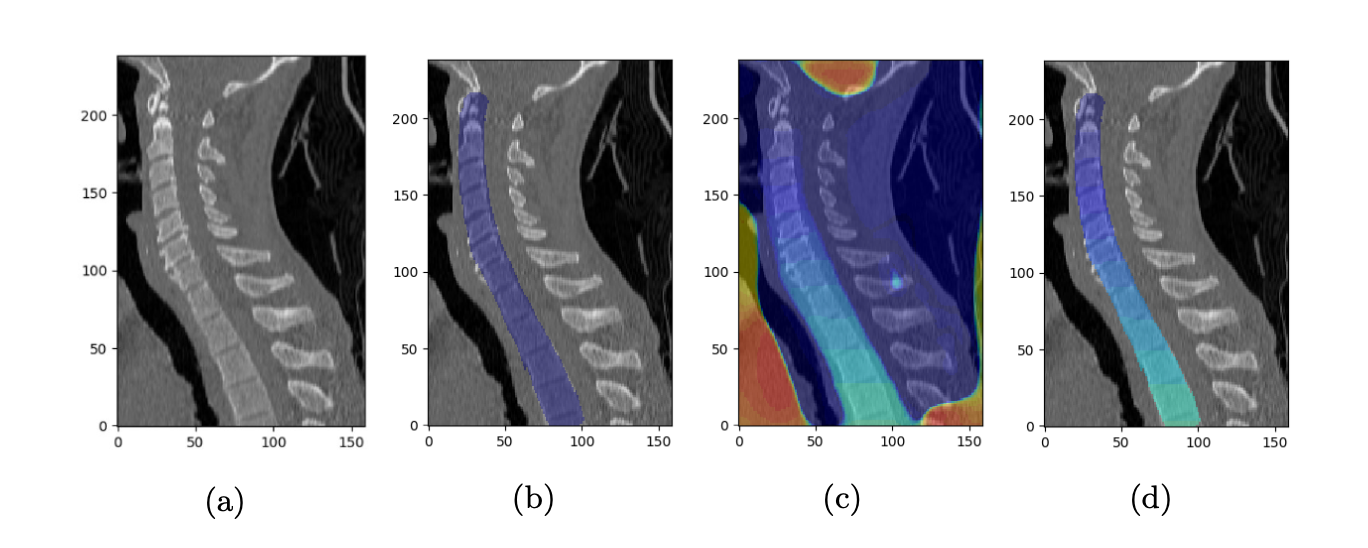
\includegraphics[width=.7\linewidth]{images/verteb_det_loc.png}
\caption {(a) shows an original scan in grey scale, (b) shows the output of the detection model applied to the scan, (c) shows the output of the identification model applied to the scan, (d) shows (b) and (c) multiplied together to produce a final prediction for each pixel.} 
\label{fig:verteb_det_loc}
\end{center}
\end{figure}

This approach was arrived at by analyzing how we could capture the ordering of the vertebrae. The identification model does not classify each pixel discretely but instead produces a continuous value for each pixel. This value is then rounded to an integer which corresponds to a specific vertebra, for example 4 = C4 vertebra. This means we can use an L1 loss function on each pixel and thus capture the ordering through this loss function. This approach would not have been possible if we had included background pixels in the identification stage therefore we segment out the background in the detection step. Our approach also captures short-range and long-range information, 3D short-range information is captured in the detection model by feeding in small 3D samples to train the network. The identification model is trained by feeding in large slices which capture long-range information, which is essential for the task of identifying individual vertebrae. To produce our final dense predictions we multiply the results of the detection model and identification model to produce a labelling on each pixel (see Figure 5.1 1d). These final predictions are then aggregated to produce final centroid estimates for each vertebra.


\subsection{Detection Model}
The detection model classifies each pixel of a scan as either ‘background’ or ‘vertebrae’1. To train the network we feed in 5 cropped samples for each scan in the training set (enforcing that at least 4 of them contain some vertebrae pixels), each sample has size 64 x 64 x 80 pixels. 

Each sample has an accompanying dense labelling, containing 0s (for background) and 1s (for vertebrae), of the same size, for the network to learn from. A 3D U-net architecture was used as portrayed in \ref{fig:detection_model_architecture}). We used a weighted categorical cross entropy loss with 2 classes as our loss function. We gave the background label a 0.1 weighting and the vertebrae label a 0.9 weighting to reflect the proportion of background labels in the samples. 
The full loss function is shown in Eq.(\ref{loss_function}) 
\begin{equation}\label{loss_function}
L(P,Q) = 0.1 * P(\theta) * \log_Q(\theta) + 0.9 * P(1)\log_Q
\end{equation}

\begin{figure}[!h]
\begin{center}
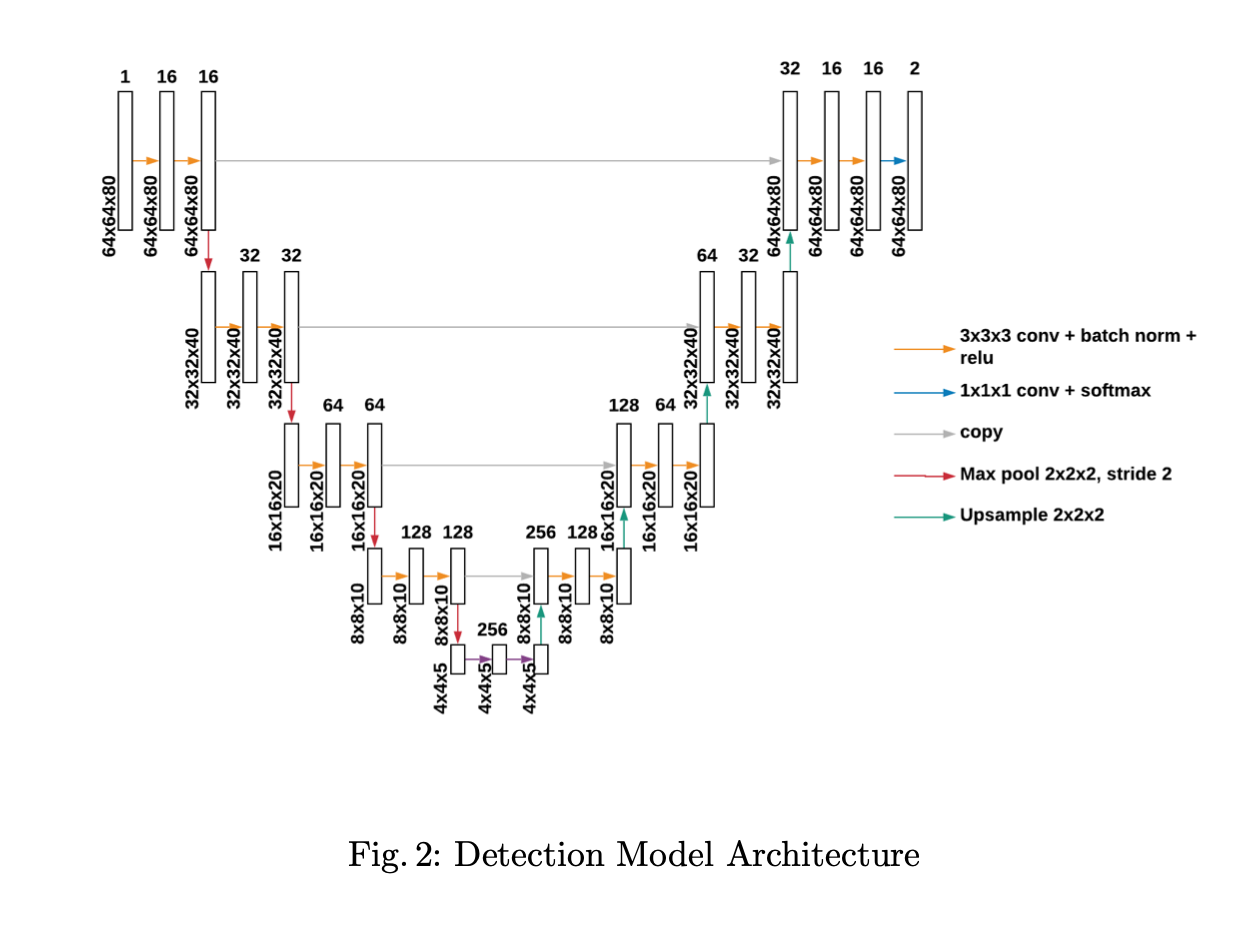
\includegraphics[width=.5\linewidth]{images/detection_model_architecture.png}
\caption {Detection Model Architecture} 
\label{fig:detection_model_architecture}
\end{center}
\end{figure}

It was used ’same’ padding for all convolutional layers with stride $1$, a learning rate $\lambda$ of $0.001$, a batch size of $16$, batch normalization after every convolutional layer with momentum of $0.1$ and trained for $50$ epochs which took $> 11$ hours on the hardware. There was obtained a validation Dice score of $0.961$ on the 1 (vertebrae) labels and a validation accuracy of 98.5\% on test samples generated from our test set.

At test time the applied detection model which scan patch-wise with some overlap between patches. The input to the network is $64 x 64 x 80$ and in steps of $32 x 32 x 40$, padding the border of the scan by $16 x 16 x 20$ and discarding the outer border of size $16 x 16 x 20$ from each output. This reduced edge artifacts in the detection and led to improved mean localization scores.

\subsection{Identification Model}
The identification model outputs a continuous value for each pixel of a scan which, is rounded to an integer to correspond to a specific vertebrae. The identification model gives a value to each pixel even if that pixel is not depicting any vertebrae and is a background. These pixels will be filtered out of the final predictions by multiplying them by their corresponding pixel from the output of the detection model which should be $0$ for a background pixel. To train the identification network it was feed in cropped samples of size $8 x 80 x 320$, generate $100$ cropped samples for each scan in the training set (enforcing that all of them capture some vertebrae pixels), each with a corresponding dense labelling of size $80 x 320$, representing the labelling for the fourth slice of the input sample. Also elastically deform each of these samples along the 2nd and 3rd axis using the elastic-deform python package. (with $\sigma$ = 0.7 on $\alpha$ $3 × 3$ grid).

It was established 2D U-net architecture for the identification model with $8$ channels in the input layer to pass in our samples of size $8 x 80 x 320$. Implemented U-net architecture with large anisotropic filters of size $5 x 20$ at the lowest level of the architecture to increase the size of the receptive field thus maximizing the contextual information captured by the network (\ref{fig:identification_model_architecture}). 

\begin{figure}[!h]
\begin{center}
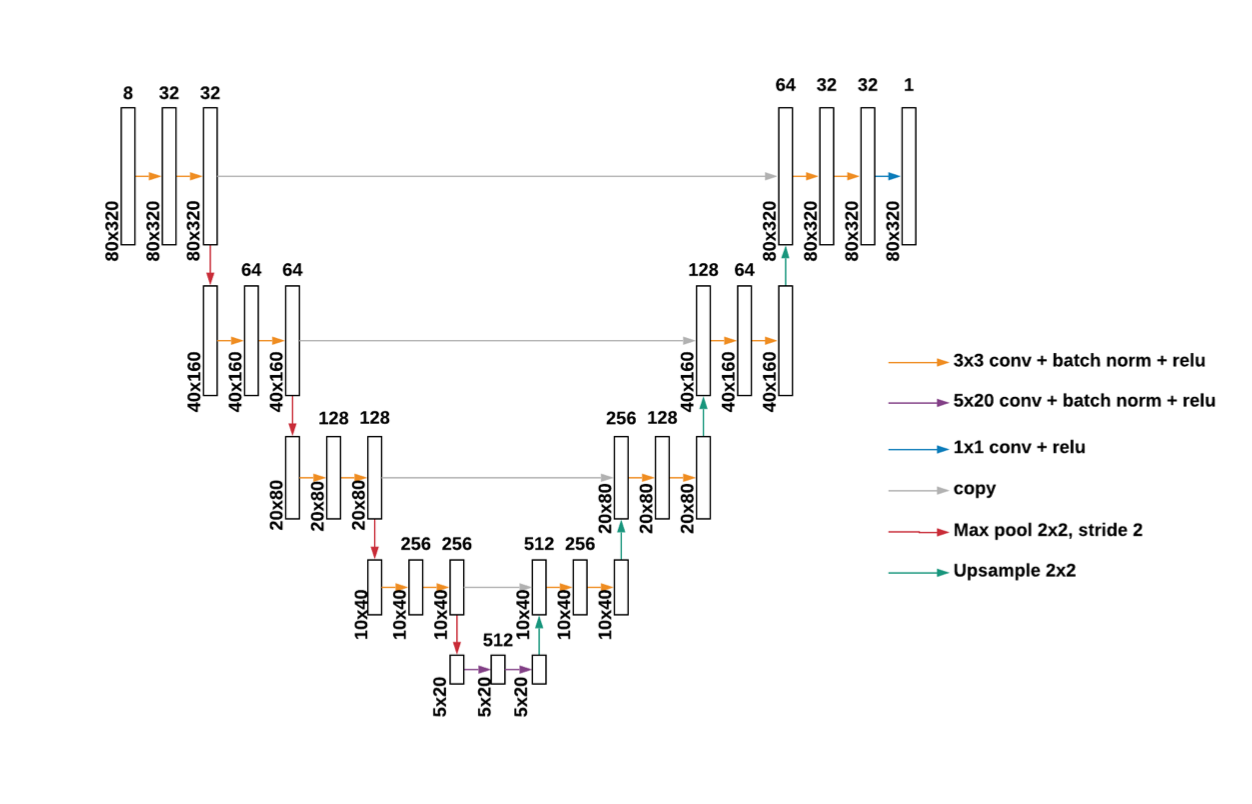
\includegraphics[width=.5\linewidth]{images/identification_model_architecture.png}
\caption {Identification Model Architecture} 
\label{fig:identification_model_architecture}
\end{center}
\end{figure}

As mentioned previously, pixels which are background will be filtered out by multiplying by the detection model. This means that we do not care about the pixels which are labelled as background when we train this model. This is reflected in the loss function which is a modified L1 loss function given below (\ref{l1_loss}):

\begin{equation}\label{l1_loss}
L = \begin{cases} \lvert $y_i$ - $x_i$ \rvert, & \mbox{if } \mbox{$x_i = 0$} \\ 
    0, & \mbox{otherwise } \end{cases}
\end{equation}
Where $y_i$ is the predicted value of pixel $i$ and $x_i$ is the true value of pixel $i$.

It was used ’same’ padding for all convolutional layers with stride $1$, a learning rate $\lambda$ of $0.001$, a batch size of $32$, batch normalization after every convolutional layer with momentum of $0.1$ and trained for $35$ epochs which took $> 7$ hours.
The identification model is a fully convolutional network which allows us to apply it to whole slices of the input scan, padded to the nearest multiple of $16$, at test time.

\subsection{Sparse to Dense Annotation}
To train both the detection and the identification model we feed in samples each with a corresponding dense labelling. In the case of the detection model the dense labelling contains two values; 0 representing background and 1 representing vertebrae (see \ref{fig:annotated_scan} b). The identification model’s dense labelling contains values from 0 to 26, 0 representing background, 1 representing C1 vertebrae etc... up to 26 representing S2 vertebrae (see \ref{fig:annotated_scan} c). Dataset comes with centroid positions (sparse labels) which must be converted to dense labels. This approach however is not the most accurate dense labelling because vertebrae are not spherical. Implemented algorithm which produces an anatomically better dense labelling, which is a better approximation of which pixels are vertebrae (detection) and which vertebra those pixels correspond to (identification), from the ground-truth sparse annotations.

The algorithm steps can be represented as:
\begin{itemize}
    \item Find midpoints between all adjacent centroids in the column.
    \item Draw line segments between these midpoints. Add additional line segments at the start and end of the column so that there is a line segment to represent
each vertebra.
    \item  Plot discs (on the plane of the sagittal and transverse axes) around each point on the line segment. The radius of these discs is specific to the vertebra the line segment represents. 
    \item Result: approximations of the radii for specific vertebrae.
\end{itemize}

\begin{figure}[!h]
\begin{center}
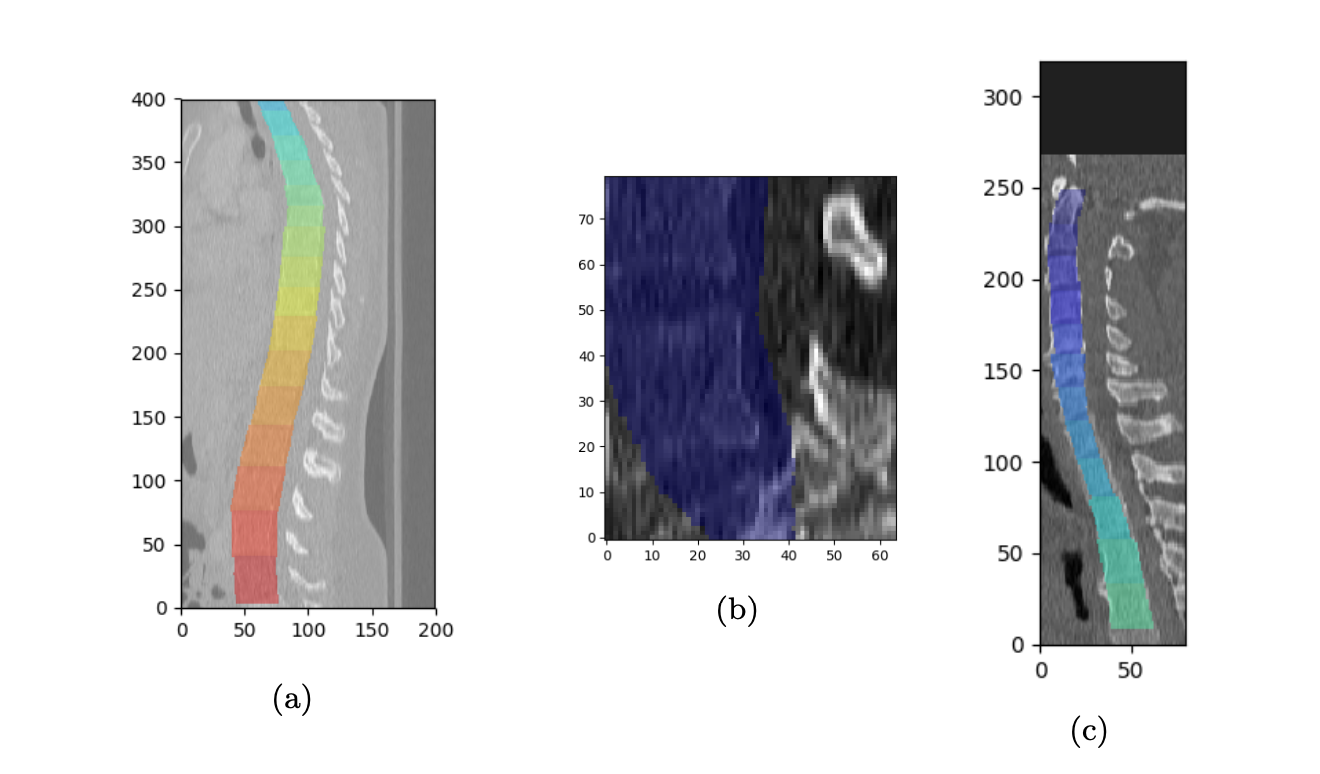
\includegraphics[width=.5\linewidth]{images/annotated_scan.png}
\caption {(a) shows a dense labelling, (b) shows an example of a sample used to train the detection model (the sample is 64 x 64 x 80 but only a 64 x 80 slice is shown here). Note: any value over 1 in the dense labelling is converted to 1 for the detection model samples, (c) shows an example of a sample used to train the identification model. Note: The size of the sample is 8 x 80 x 320, if the original scan is not larger enough to fill those dimensions some padding is added, as can be seen at the top.} 
\label{fig:annotated_scan}
\end{center}
\end{figure}


\subsection{Dense to Sparse Annotation}
Once a label has been predicted for each pixel (see \ref{fig:verteb_det_loc} d) these labels are aggregated to calculate predicted centroid positions. To aggregate we find the median position of all pixels which vote for each vertebra. However before calculating this we apply a threshold so that if there are less than a certain number of pixels voting for a vertebra we do not include that centroid in the prediction. This filters out erroneous predictions produced by the identification model.
The threshold $x_v$ is specific to the vertebra $v$ and is calculated using Eq.\ref{x_v threshold}

\begin{equation}\label{x_v threshold}
x_v = max(3000, 0.4R_v^3)
\end{equation}
where $R$ is the radius of the vertebra $v$. 